
\documentclass[12pt,fleqn,leqno,letterpaper]{article}
\usepackage[utf8]{inputenc}
\usepackage[english]{babel}

\usepackage{hyperref}
\usepackage{graphicx}
\usepackage{minted}

\include{preamble}


\title{Assignment 1}
\author{Anders L. Hurum\\
    \small{Development of Real-Time Systems}\\
    \small{EIT Digital}\\
    \small{Assignment 1}\\
    \small{\texttt{andershurum@gmail.com}}
}
\date{September 11, 2017}

\begin{document}


    \maketitle

    \begin{abstract}
        
        The first assignment for the course consisted of creating tasks in FreeRTOS, 
        and getting those tasks to run with different delays and priorities.  
        Further the tasks should have a seperate debug message each. \\ \\
        For more details on the assignment, see the \texttt{assignment\_1.md} document 
        in the repository at github. \\
        
        \url{http://github.com/peakbreaker/tuts\_FreeRTOS}

    \end{abstract}

    \newpage

    \section*{Code}

        The main function:

        \begin{minted}{c}
            int main(void)
            {
                /* Initializations for heap and trace recorder */
                prvInitialiseHeap();    
                vTraceInitTraceData();
                xTickTraceUserEvent = xTraceOpenLabel("tick");
            
                /* Create the tasks */
                xTaskCreate(Task1, "Task1", 1000, 100, 3, NULL);
                xTaskCreate(Task2, "Task2", 100, 500, 1, NULL);
                
                // This starts the real-time scheduler
                vTaskStartScheduler();
                
                // Should not reach here
                for ( ;; );
                
                return 0;
            }
        \end{minted}

        One of the tasks:

        \begin{minted}{c}
            void Task1(int msDelay) {
                // Block for the defined time
                const TickType_t xDelay = msDelay / portTICK_PERIOD_MS;
            
                for ( ;; ) {
                    // Print the message and do the delay
                    printf("This is task 1");
                    fflush(stdout);
                    vTaskDelay( xDelay );
                }
            }
        \end{minted}

        For the assignment I edited the main.c file.  I created two tasks which takes an integer (delay time) as an argument.
    \newpage
    \section*{Results}

        The resulting output from the program were as follows : \\

        \begin{figure}[h]
            \centering
            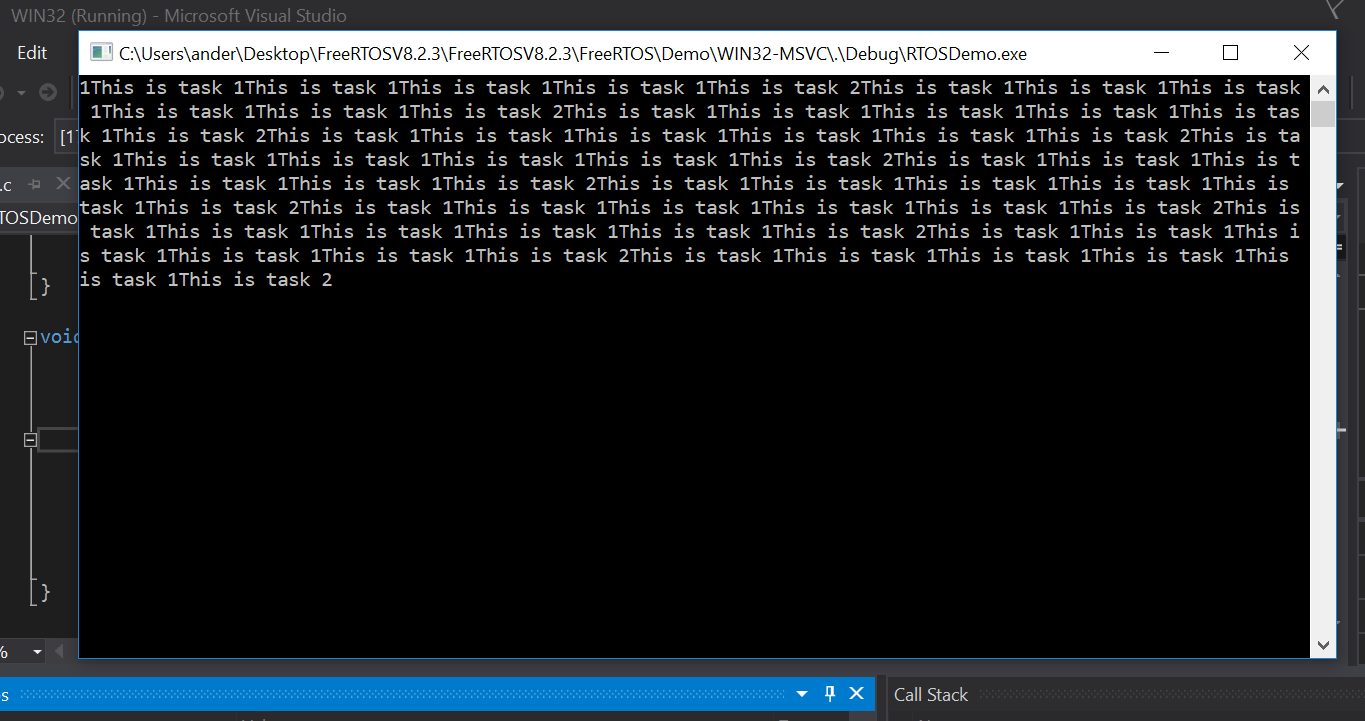
\includegraphics[width=\textwidth]{Debug.png}
            \caption{Debug output}
            \label{figure:debug}
        \end{figure}

        As the output shows, Task1 debugs out five times as often as Task2.  This meets the specified requirements for the assignment (Task 1 output every 100 ms, Task 2 output every 500 ms).\\
        
        The repository for the entire assignment can be found at my github : \\
        
        \url{http://github.com/peakbreaker/tuts\_FreeRTOS}

    \end{document}